\documentclass[11pt,a4paper]{article}
\usepackage{graphicx}
\usepackage{float}
\usepackage{hyperref}
\usepackage{listings}
\usepackage[margin=2cm]{geometry}
\raggedbottom
\graphicspath{{../screenshots/}}
\lstset{basicstyle=\ttfamily\small,breaklines=true,frame=single}
\title{Wazuh SIEM Homelab: Single-Node Detection Lab}
\author{Nizami Hasanov}
\date{September 2026}

\begin{document}
\maketitle

\section{Goal and Architecture}
The goal of this lab was to build a working SIEM detection pipeline and prove
it end to end: generate an attack, collect the logs, fire a stock rule, then
write and validate a custom detection. The stack is the official Wazuh
single-node Docker deployment (version 4.14.8): one manager, one indexer, one
dashboard, plus a Dockerized Ubuntu victim with an enrolled Wazuh agent.
The detection scenario covers SSH password guessing, mapped to MITRE
T1110.001 (Brute Force: Password Guessing).

\begin{lstlisting}
attacker (host) --> victim-ubuntu (sshd, agent)
victim-ubuntu --auth.log--> manager:1514
manager --filebeat--> indexer:9200 --> dashboard:443
\end{lstlisting}

\section{Build: Single-Node Stack}
I followed the official single-node Docker guide: cloned
\texttt{wazuh-docker}, generated indexer certificates with the
\texttt{wazuh-certs-generator} container, and started the stack with
\texttt{docker compose up -d}. The host (Arch Linux, 8 GB RAM) already
exceeded the indexer memory-map requirement, and the required ports
(443, 9200, 1514, 1515) were free.
First boot took about two minutes while the indexer built its indexes; cluster
health reported \texttt{green} with one node.

\begin{figure}[H]\centering
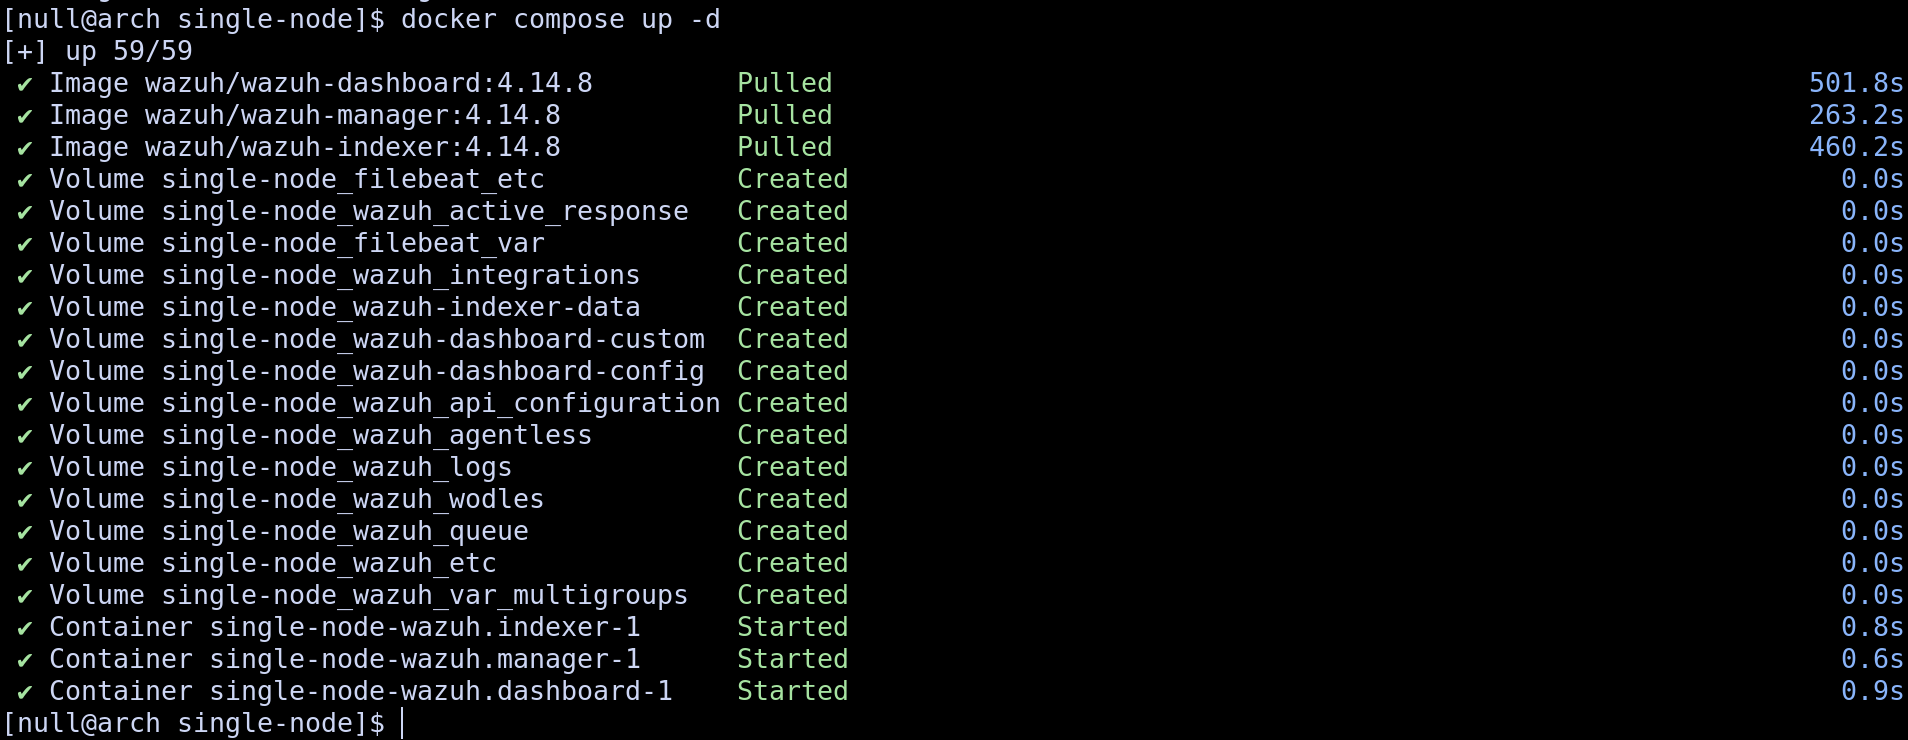
\includegraphics[width=\textwidth,height=0.6\textheight,keepaspectratio]{02-stack-boot.png}
\caption{Stack boot: images pulled, volumes created, all three containers started}
\end{figure}
\begin{figure}[H]\centering
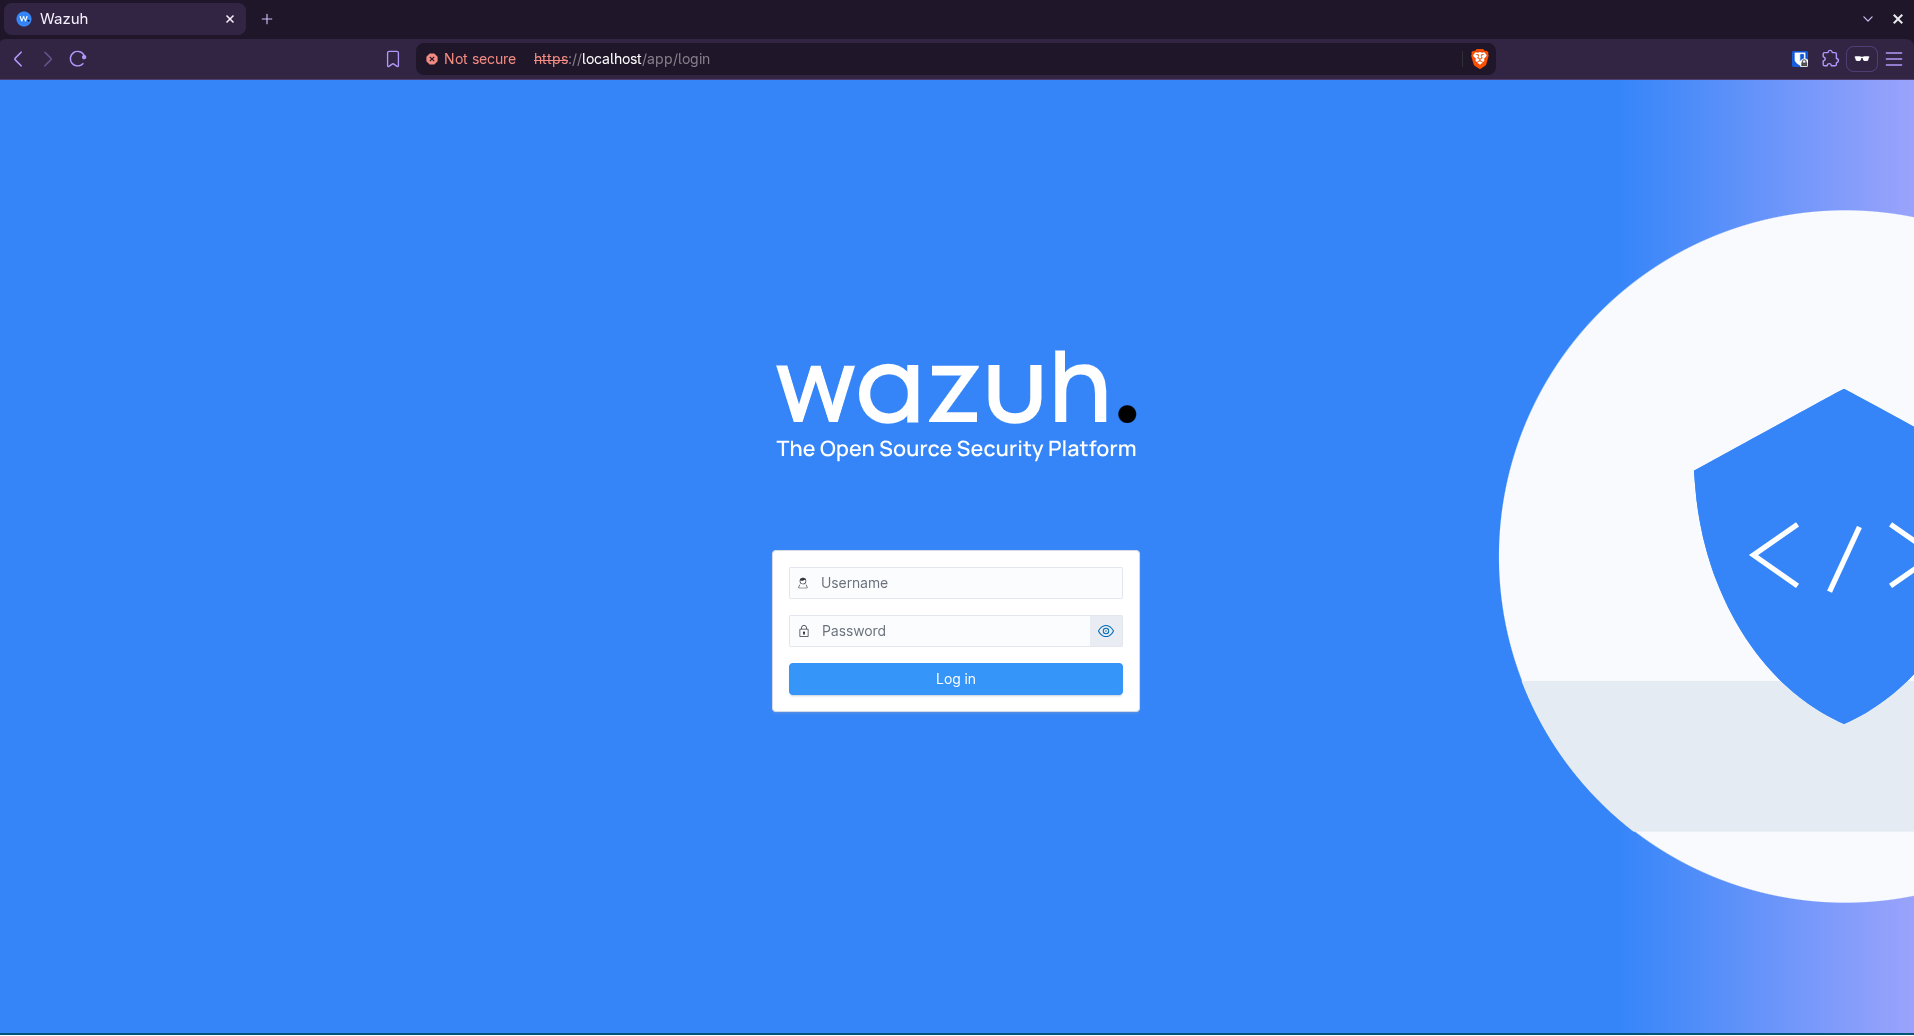
\includegraphics[width=\textwidth,height=0.6\textheight,keepaspectratio]{01-dashboard-login.png}
\caption{Dashboard reachable at https://localhost}
\end{figure}

\section{Victim Enrollment}
The victim is an \texttt{ubuntu:22.04} container named
\texttt{victim-ubuntu}, attached to the compose network
\texttt{single-node\_default} so the manager hostname
\texttt{wazuh.manager} resolves. Inside it I installed the Wazuh agent
(4.14.8, matching the manager) and OpenSSH server. Two issues came up:
the agent ships with the placeholder \texttt{MANAGER\_IP} in
\texttt{ossec.conf}, which I replaced with \texttt{wazuh.manager}, and
enrollment is passwordless on this manager (\texttt{use\_password=no}),
so \texttt{agent-auth -m wazuh.manager -A victim-ubuntu} was enough.
The manager then listed the agent as \texttt{ID 001, Active}.

\begin{figure}[H]\centering
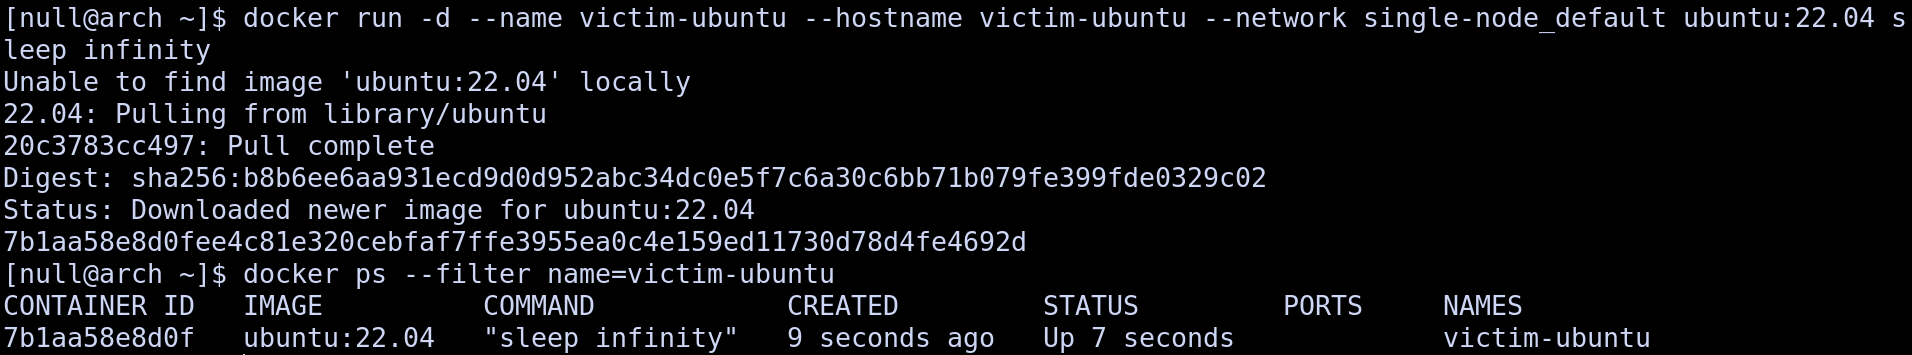
\includegraphics[width=\textwidth,height=0.6\textheight,keepaspectratio]{03-victim-launch.png}
\caption{Victim container launch: image pull and running status}
\end{figure}
\begin{figure}[H]\centering
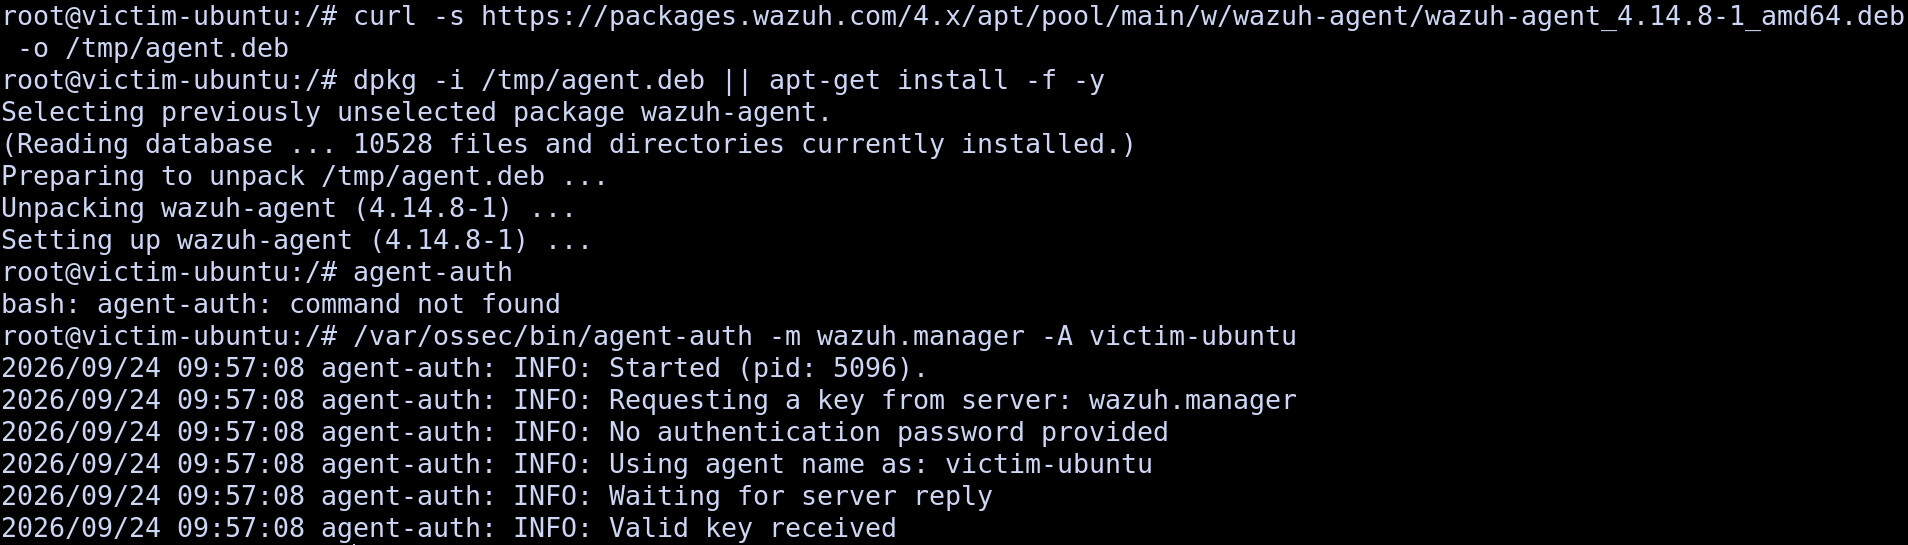
\includegraphics[width=\textwidth,height=0.6\textheight,keepaspectratio]{04-agent-install-enroll.png}
\caption{Agent package install and passwordless enrollment (valid key received)}
\end{figure}
\begin{figure}[H]\centering
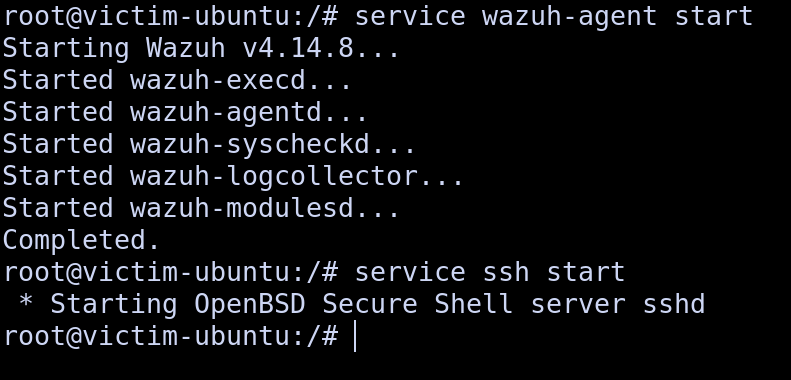
\includegraphics[width=\textwidth,height=0.6\textheight,keepaspectratio]{05-agent-services-start.png}
\caption{Agent and SSH services started on the victim}
\end{figure}
\begin{figure}[H]\centering
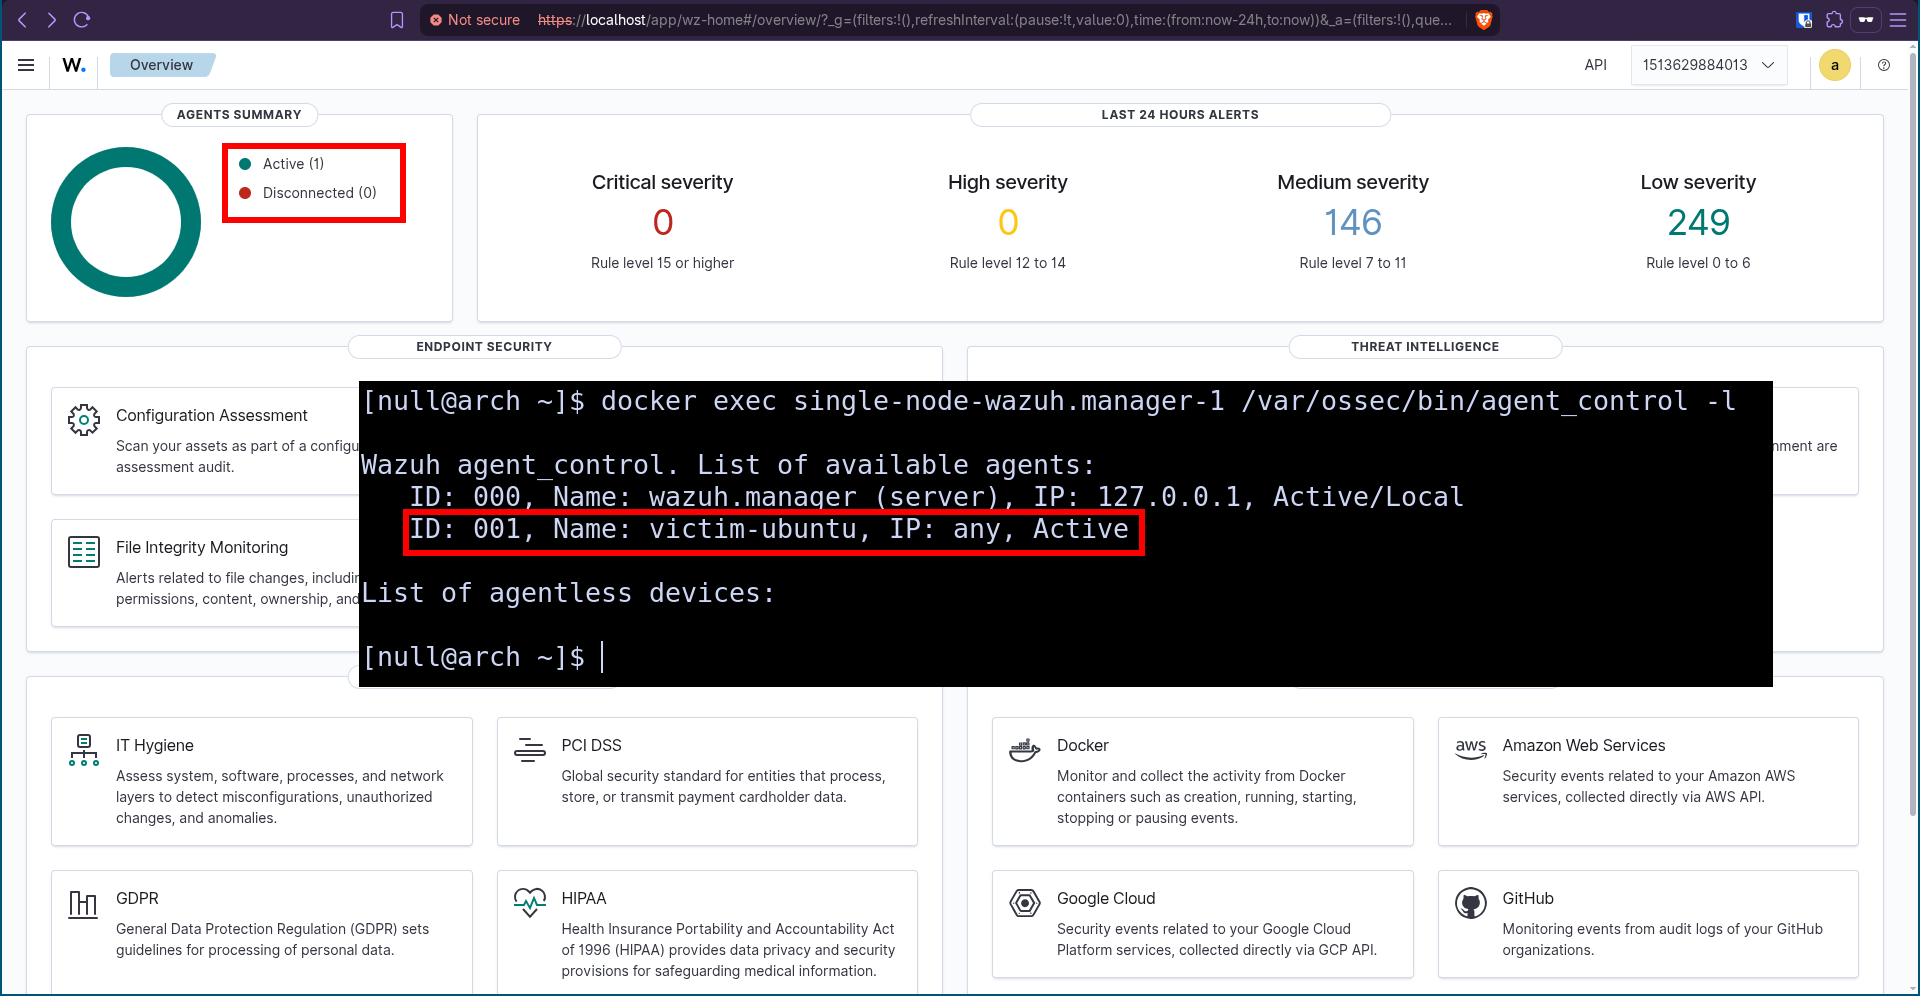
\includegraphics[width=\textwidth,height=0.6\textheight,keepaspectratio]{06-agent-active.png}
\caption{Agent 001 Active: dashboard overview (1 active, alert counters) and manager CLI}
\end{figure}

\section{Problem: Missing Auth Logs}
The first brute force produced no alerts. Debugging showed the attack did
reach the victim (orphaned \texttt{sshd} processes at the attack time) but
was logged nowhere: the container ships without a syslog daemon, so
\texttt{/var/log/auth.log} did not exist, and the agent's \texttt{journald}
source reads nothing without systemd. The fix was to install rsyslog and run
\texttt{rsyslogd} directly (no init system in the container, so
\texttt{service rsyslog start} didn't work), then add a file monitor to the
agent configuration (Figure 7):

\begin{lstlisting}
<localfile>
  <log_format>syslog</log_format>
  <location>/var/log/auth.log</location>
</localfile>
\end{lstlisting}

After restarting the agent, failed logins appeared in \texttt{auth.log} and
flowed to the manager.

\begin{figure}[H]\centering
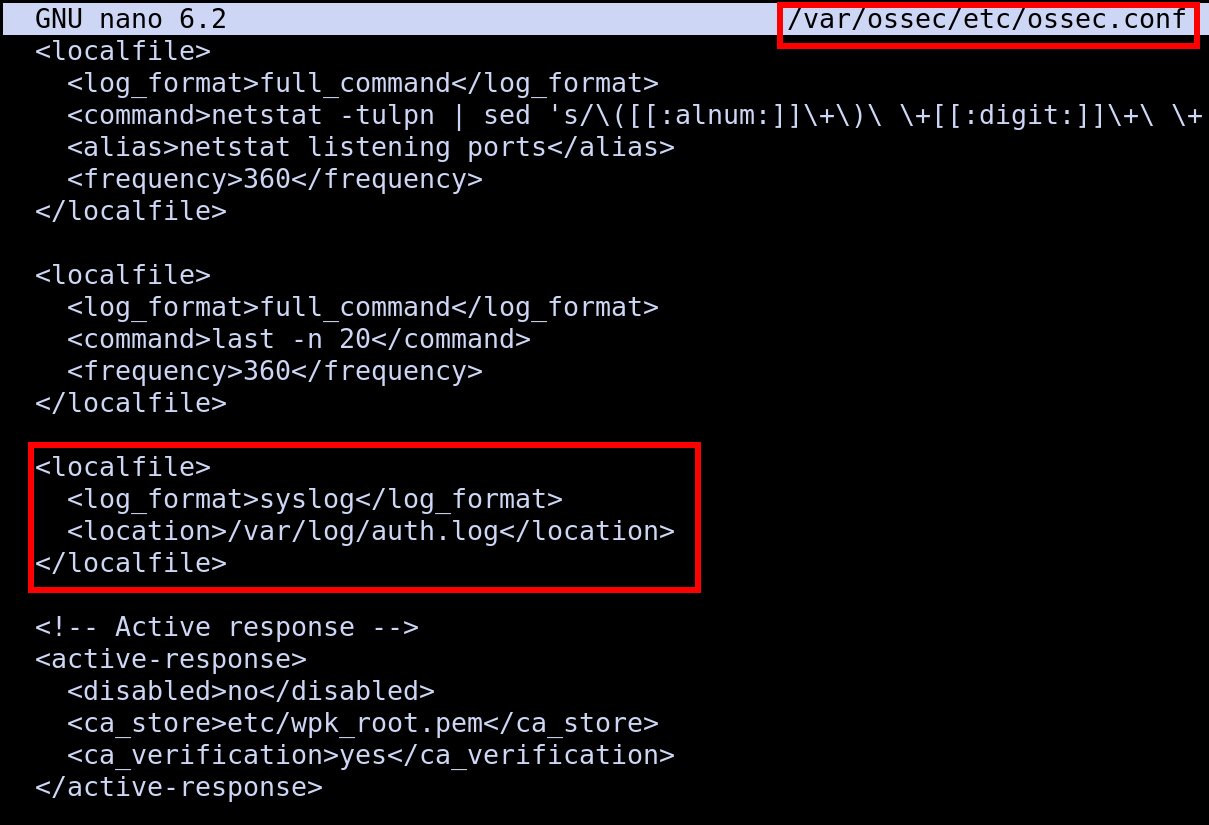
\includegraphics[width=\textwidth,height=0.6\textheight,keepaspectratio]{07-ossec-authlog-config.png}
\caption{auth.log file monitor added to the agent ossec.conf}
\end{figure}

\section{Detection 1: Stock Rule (Password Guessing)}
The attack is a minimal password loop from the host against the victim's IP:

\begin{lstlisting}
for i in 1 2 3 4 5 6 7 8; do
  sshpass -p x ssh -o StrictHostKeyChecking=no fakeuser@VICTIM_IP exit
done
\end{lstlisting}

Each attempt logs \texttt{Failed password for invalid user}, which fires
stock rule \textbf{5710} (level 5, ``Attempt to login using a non-existent
user'') rather than the generic 5716, because the message names an invalid
user. PAM failures fire \textbf{5503}, and bursts also trip the stock
aggregate \textbf{5551} (level 10, multiple failed logins). A repeat run
confirmed the alerts land in Threat Hunting within about a minute.

\begin{figure}[H]\centering
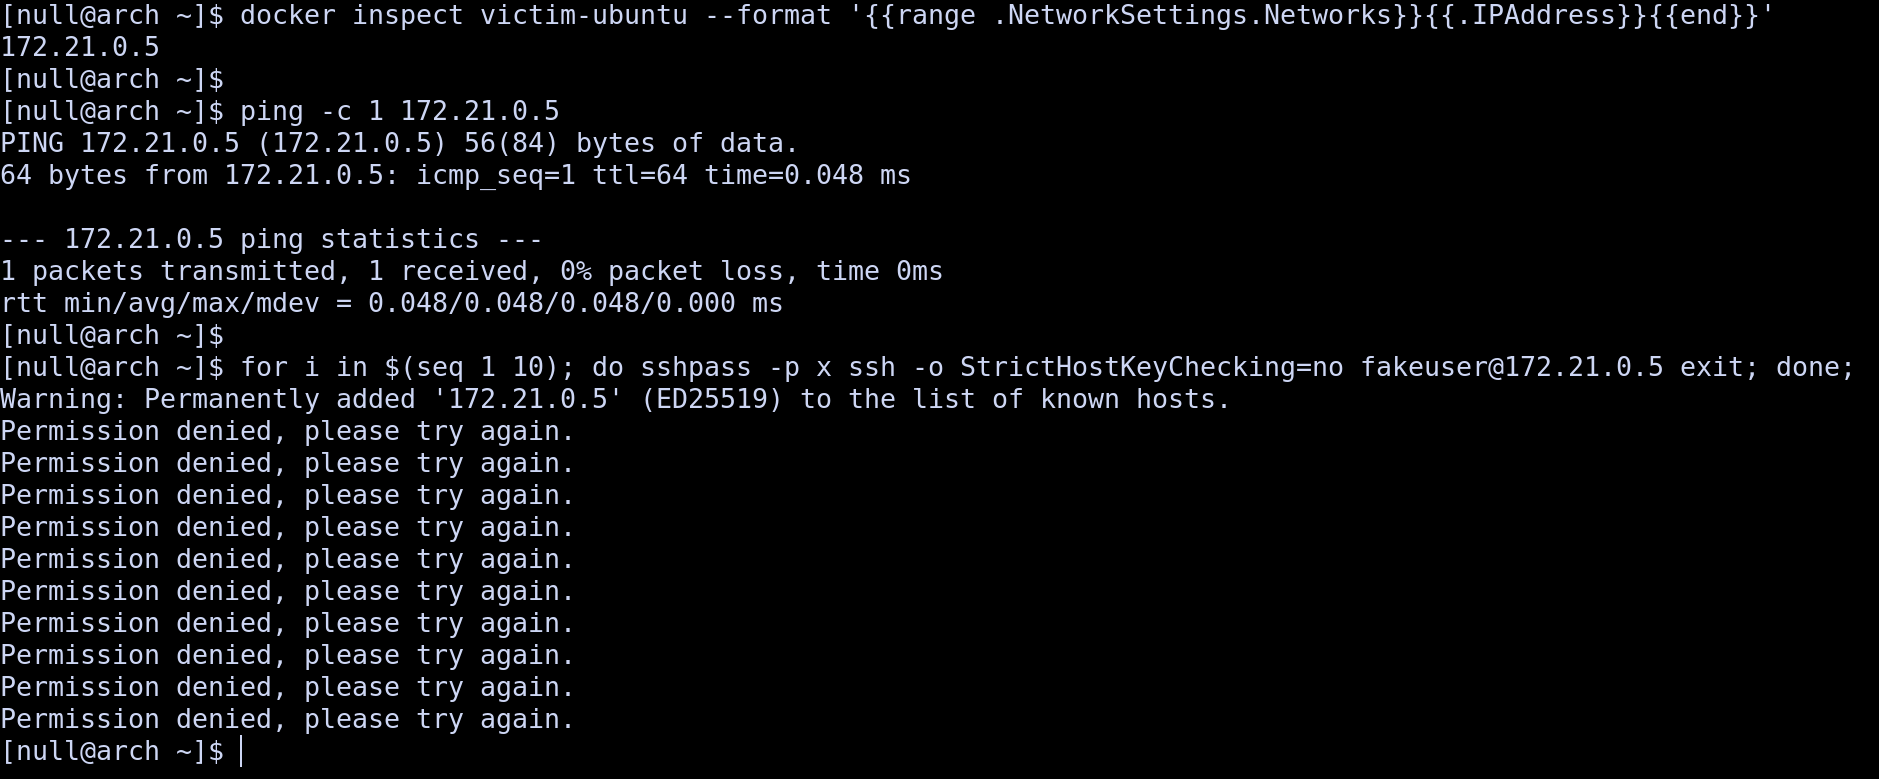
\includegraphics[width=\textwidth,height=0.6\textheight,keepaspectratio]{08-first-bruteforce.png}
\caption{First brute-force loop and resulting auth.log traces on the victim}
\end{figure}
\begin{figure}[H]\centering
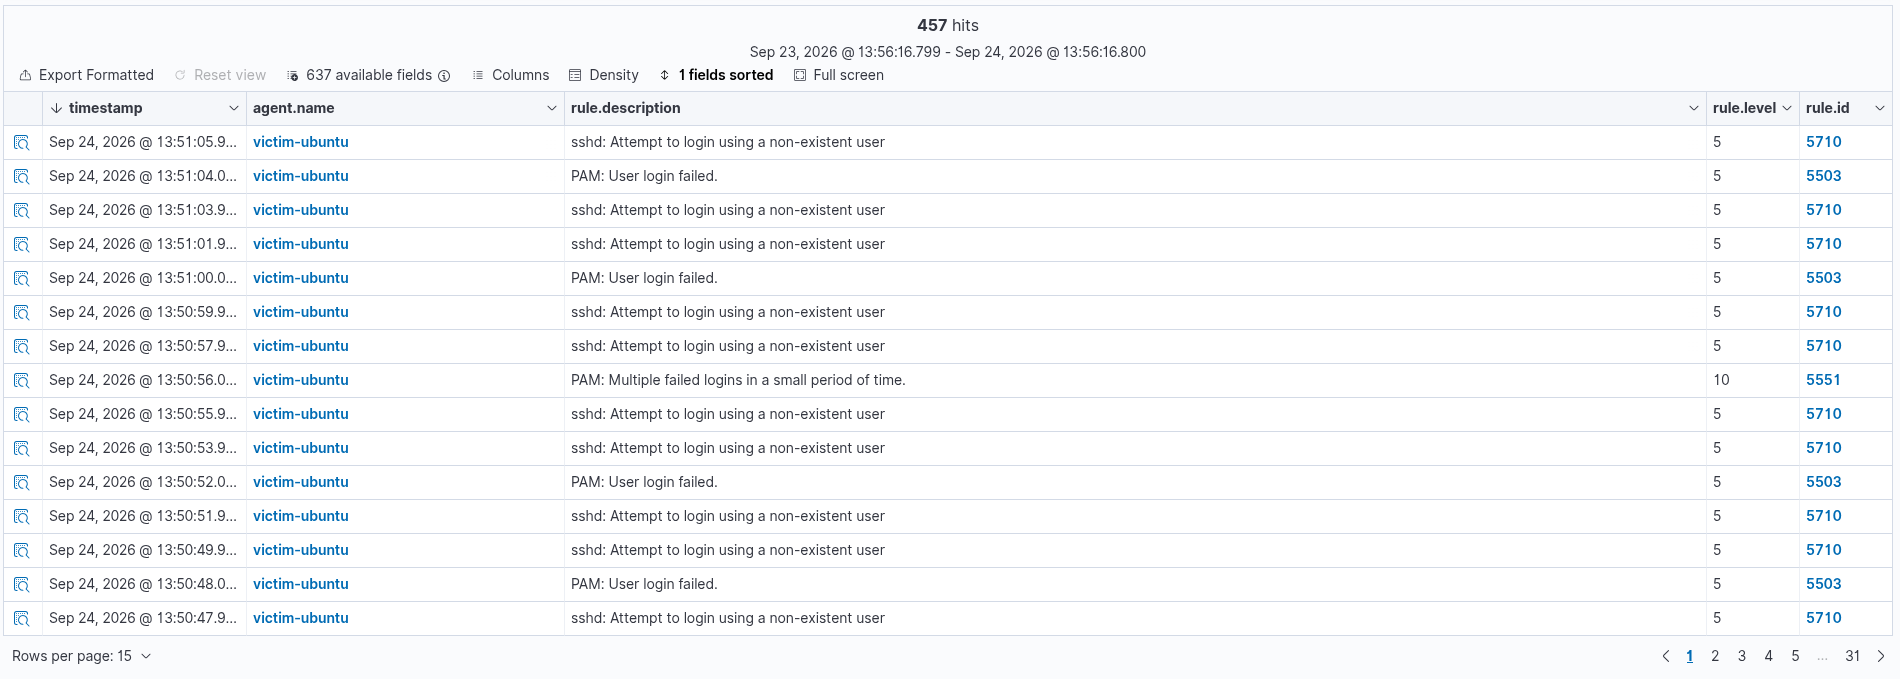
\includegraphics[width=\textwidth,height=0.6\textheight,keepaspectratio]{09-stock-5710-alerts.png}
\caption{Stock detections for the victim: 5710, 5503, and aggregate 5551}
\end{figure}
\begin{figure}[H]\centering
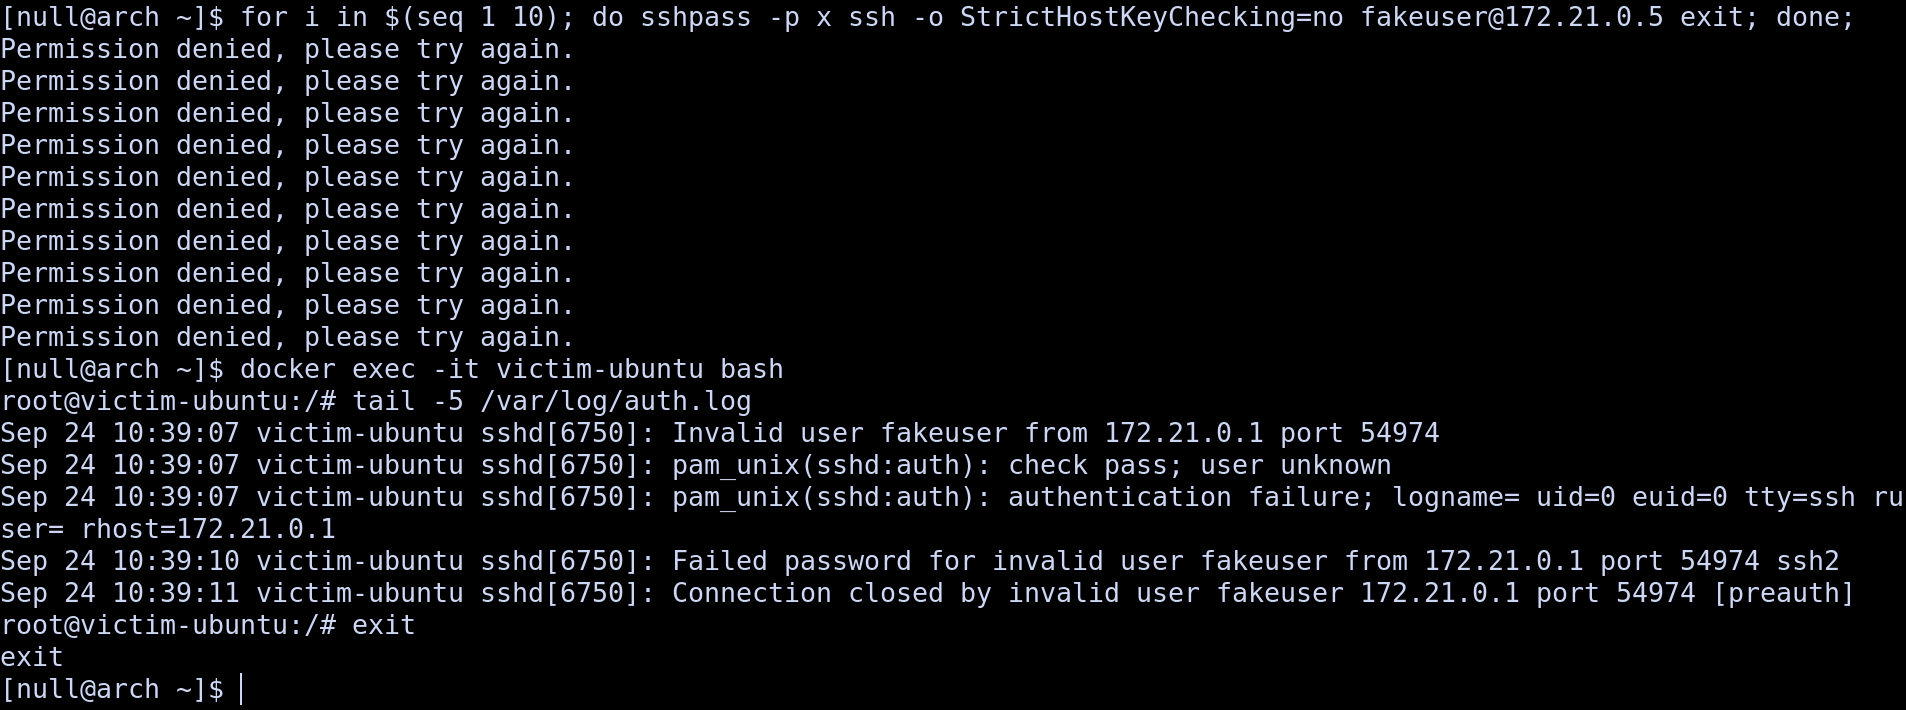
\includegraphics[width=\textwidth,height=0.6\textheight,keepaspectratio]{10-second-bruteforce.png}
\caption{Repeat run against the victim IP for custom-rule validation}
\end{figure}

\section{Detection 2: Custom Rule 100100}
A per-attempt level-5 alert is noise; the SOC-relevant signal is the
aggregate: 5 failures in 60 seconds at level 10, tagged T1110.001. I created
the rule in the dashboard editor (Management $\rightarrow$ Rules $\rightarrow$
Files $\rightarrow$ \texttt{local\_rules.xml}):

\begin{lstlisting}
<group name="homelab,">
  <rule id="100100" level="10" frequency="5" timeframe="60">
    <if_matched_sid>5710</if_matched_sid>
    <description>SSH brute force, 5 fails in 60s</description>
    <mitre><id>T1110.001</id></mitre>
  </rule>
</group>
\end{lstlisting}

Two syntax failures preceded the working version, both caught by
\texttt{wazuh-analysisd -t} (warning 7615, rule ignored): first a
comma-plus-space list in \texttt{if\_matched\_sid}, then a spaceless list.
\texttt{if\_matched\_sid} accepts exactly one rule ID, so the final rule
watches 5710 only, which matches this scenario since every attempt targets a
nonexistent user. After a manager restart and a fresh brute force, rule
100100 fired at level 10 (fired 4 times in the test window).

\begin{figure}[H]\centering
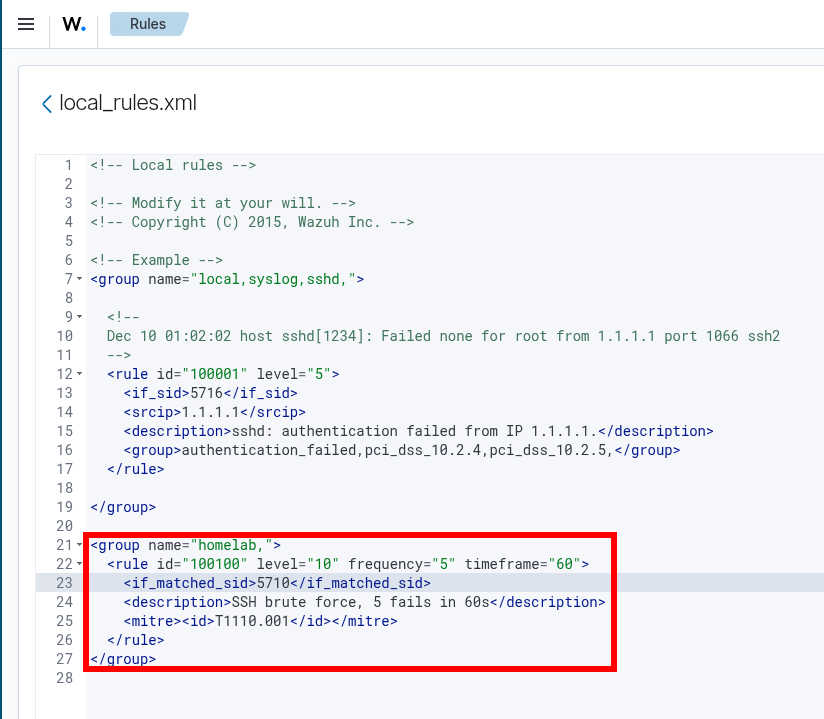
\includegraphics[width=\textwidth,height=0.6\textheight,keepaspectratio]{11-custom-rule-editor.png}
\caption{Custom rule 100100 in the dashboard ruleset editor}
\end{figure}
\begin{figure}[H]\centering
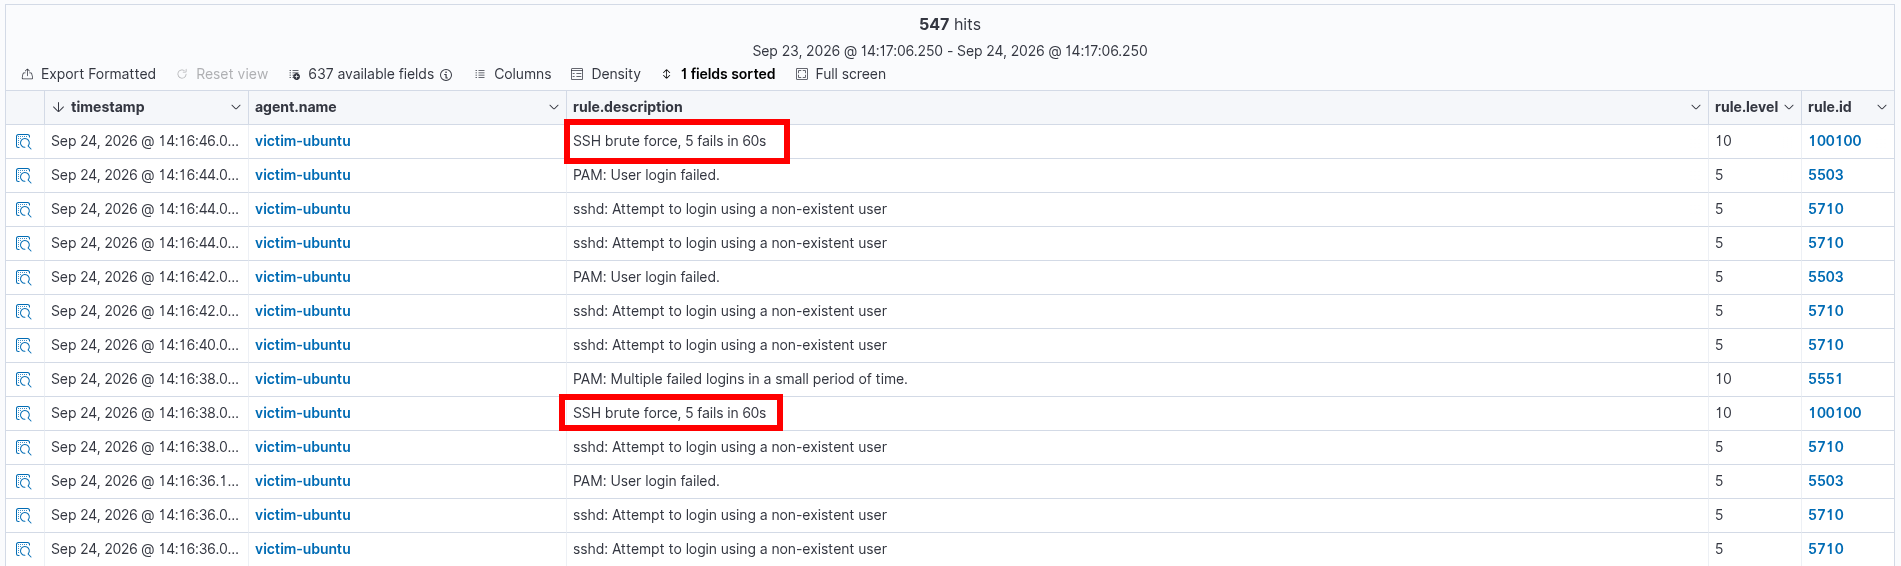
\includegraphics[width=\textwidth,height=0.6\textheight,keepaspectratio]{12-custom-100100-alerts.png}
\caption{Custom rule 100100 fired at level 10 alongside stock rules}
\end{figure}
\begin{figure}[H]\centering
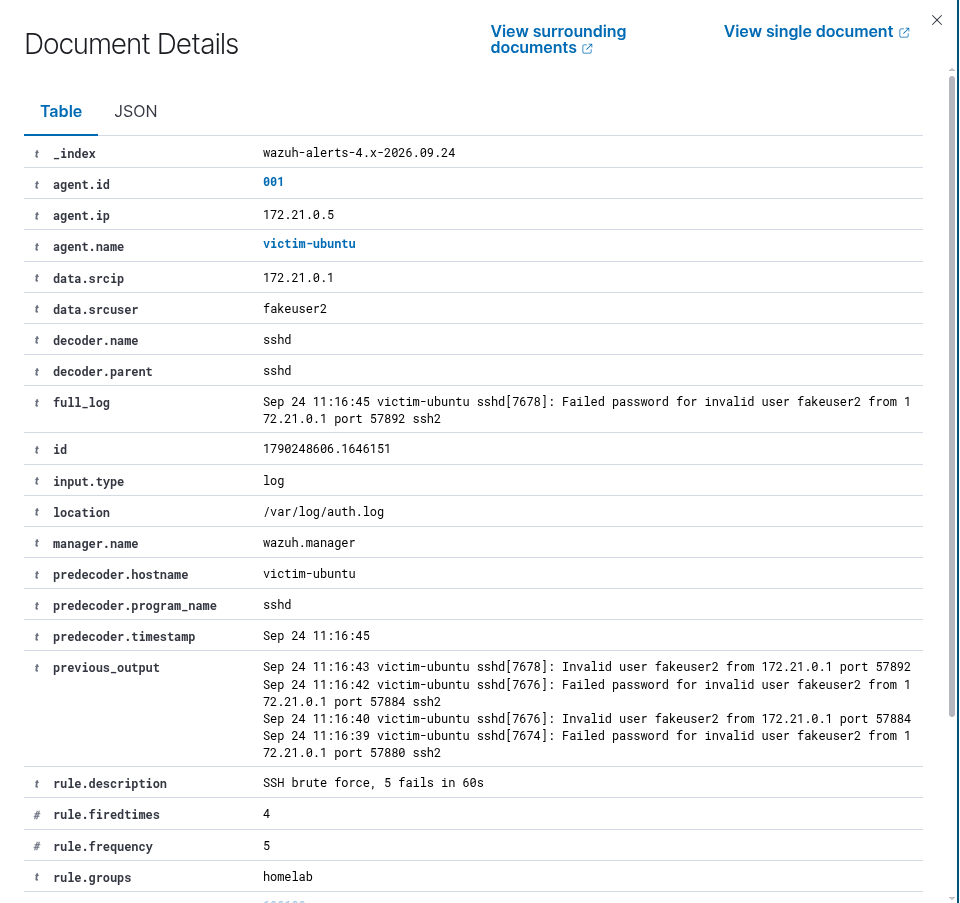
\includegraphics[width=\textwidth,height=0.6\textheight,keepaspectratio]{13-custom-alert-detail.png}
\caption{Alert detail: victim-ubuntu agent, attacker source IP, MITRE tag, frequency 5}
\end{figure}

\subsection{Threshold rationale}
A human mistypes roughly 1--3 passwords, then succeeds or stops; scripted
guessing does dozens per minute. Five failures in 60 seconds catches
automation fast in a quiet lab without flagging one fat-fingered session.
The stock sshd aggregate (5712) uses 8 in 120 seconds --- stricter, tuned
for busy servers. The 5/60 choice validates faster against a near-zero
baseline. Rule source is committed as \texttt{detections/local\_rules.xml}.

\subsection{False positives}
Known false positives: a legitimate user retrying five times in a minute
(wrong keyboard layout, expired password) raises a level-10 alert on a
human --- mitigate with allowlists or by correlating with a subsequent
successful login. Automation with a stale key (ansible, CI, monitoring
logins) retrying on schedule --- mitigate by allowlisting automation source
IPs. Accepted scope flaw: the rule has no \texttt{same\_source\_ip}, so the
count is global across agents; five users failing once each on five hosts
would fire it. Acceptable with one victim, but production needs per-source
scoping. There is also no \texttt{ignore} window, so a sustained brute
force emits one alert per five events (four fired in the test run); add
\texttt{ignore="60"} after tuning. Tuning loop: run one week, compare rule
100100 hits against confirmed incidents, then adjust frequency and
timeframe.

\section{MITRE Mapping}
\begin{center}
{\small
\begin{tabular}{@{}lll@{}}
\hline
Rule & Event & Technique \\
\hline
5710 & Invalid-user SSH login failure (stock) & T1110.001 \\
5503 & PAM authentication failure (stock) & T1110.001 \\
5551 & Multiple failed logins, small period (stock) & T1110.001 \\
100100 & 5 SSH failures in 60s (custom) & T1110.001 \\
\hline
\end{tabular}
}
\end{center}

\section{Next Steps}
Planned extensions: file integrity monitoring on \texttt{/etc} of the
victim, an active-response block on brute-force sources, a second scenario
(unauthorized \texttt{sudo} attempts), and a Windows agent for cross-platform
coverage.

\end{document}
